\begin{frame}{Mesurer le degré d'intertextualité}

{\small(\textit{Traductologie}) Mesurer l'influence d'un écrivain sur le style de son traducteur {\footnotesize(\cite{oseki2007})}.}
\\
$\rightarrow$ mesurer informatiquement l'impact de Charcot sur son réseau
\begin{itemize}
\item analyse des concepts-clés médicaux
\item intertextualité uni-directionnelle {\small\textsc{Charcot}} $\rightarrow$ {\small\textsc{Autres}}
\end{itemize}
\begin{figure}[!h]
    \centering
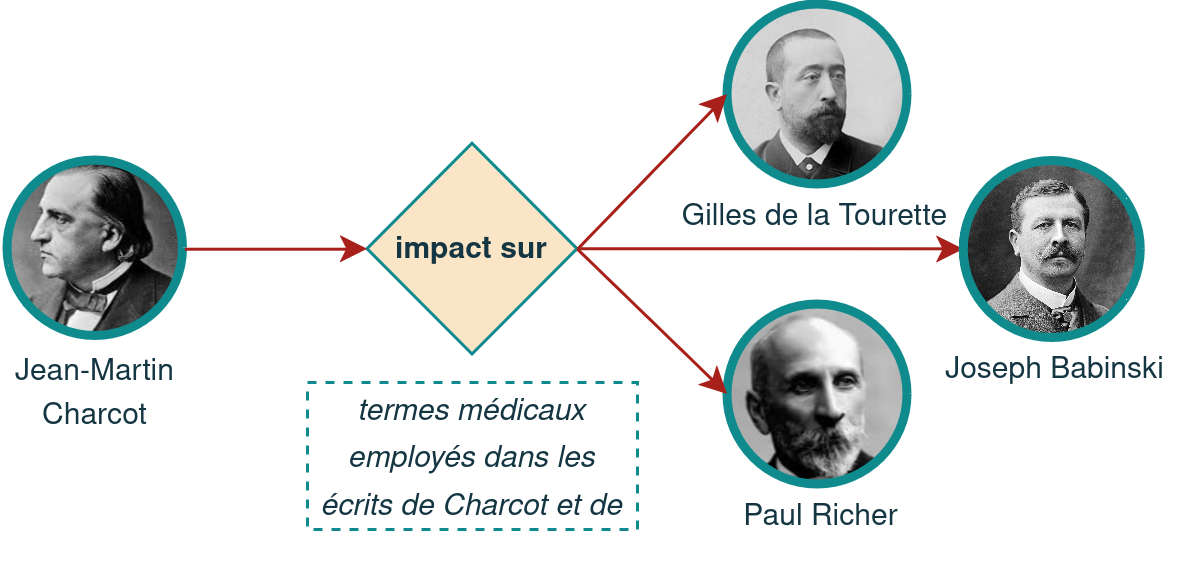
\includegraphics[width=85mm,scale=0.5]{pic/charcot_intertextualite.png}
    \caption{Opérationnalisation de l'impact de Charcot sur ses élèves.}
    \label{fig:my_label}
\end{figure}
\end{frame}

